\chapter{प्रावस्था संक्रमण}\label{ch:b3:phase-transitions}

पानी को एक अंश गरम कीजिए, कुछ खास नहीं होता --- जब तक कि किसी एक
तीखे ढंग से परिभाषित ताप पर वह द्रव स्वयं को चीरकर वाष्प न बना ले।
लोहे को \qty{1043}{K} से नीचे ठंडा कीजिए और, बिना किसी संघटन-परिवर्तन
के, वह स्वतःस्फूर्त रूप से चुंबकित हो जाता है। किसी एक अणु या किसी एक
चक्रण में इन क्रांतियों की कोई घोषणा नहीं होती: वे \emph{सामूहिक} हैं
--- $10^{23}$ कर्ता, जिनमें से हर एक कुछ ही पड़ोसियों से
अन्योन्यक्रिया करता है, और सब मिलकर अपने समाज की प्रावस्था एक ही साथ
बदल डालते हैं। वर्ष 1 के खंड ने संक्रमणों की सूची बनाई थी; यह अध्याय
पिछले पाँच अध्यायों के औज़ारों से उनकी क्रियाविधि समझाता है:
मुक्त-ऊर्जा की होड़, \omterm{def:b3:phase-transitions:order}{क्रम-प्राचल}, सममिति का भंग, और वह चकित करने
वाली खोज कि किसी \omterm{prop:b3:phase-transitions:vdw}{क्रांतिक बिंदु} के पास सूक्ष्म ब्योरे मायने रखना बंद
कर देते हैं --- कोई चुंबक और कोई उबलता तरल एक ही \omterm{prop:b3:phase-transitions:landau}{क्रांतिक चरघातांक}
साझा करते हैं। इस अध्याय के विचार आज प्रेशर कुकर से लेकर अतिचालकों
तक और \cref{ch:b3:particle-physics} के हिग्स क्षेत्र तक चलते हैं।

\section{क्रम-प्राचल और मुक्त-ऊर्जा की होड़}

\begin{definition}[प्रावस्थाएँ और क्रम-प्राचल]\label{def:b3:phase-transitions:order}
\index{प्रावस्था संक्रमण}\index{क्रम-प्राचल}\index{सममिति-भंग}
कोई \emph{प्रावस्था संक्रमण} किसी तंत्र की संतुलन-अवस्था का वह
अ-चिकना परिवर्तन है, जो तब होता है जब कोई नियंत्रण-प्राचल ($T$, $P$,
$B$) किसी सीमा को पार करे। उसका हिसाबी है \emph{क्रम-प्राचल}: वह राशि
जो अव्यवस्थित प्रावस्था में शून्य और व्यवस्थित में अशून्य होती है ---
किसी लौहचुंबक का चुंबकन $m$, किसी तरल का घनत्व-अंतर
$\rho_{\text{द्र}} - \rho_{\text{गै}}$, या
\cref{ch:b3:quantum-statistics} का संघनित अंश। संक्रमण दो तरह के
होते हैं: \emph{प्रथम-कोटि} (क्रम-प्राचल छलाँग लगाता है; गुप्त ऊष्मा;
प्रावस्थाएँ साथ रहती हैं --- उबलना, गलना) और \emph{सतत} (क्रम-प्राचल
शून्य से बढ़ता है; कोई गुप्त ऊष्मा नहीं; उन्मत्त उतार-चढ़ाव ---
क्यूरी बिंदु, \omterm{prop:b3:phase-transitions:vdw}{क्रांतिक बिंदु}, अतितरल हीलियम)। जब व्यवस्थित अवस्था को
तुल्य विकल्पों में से \emph{चुनना} ही पड़े --- किसी चुंबक के उत्तर को
कहीं तो इशारा करना ही है --- तब वह संक्रमण उस \emph{सममिति को भंग}
करता है, जिसका आधारभूत नियम आदर करते हैं: यही विषय, सबसे ऊँचे दाँव
पर, हिग्स क्रियाविधि के साथ लौटेगा।
हर स्थिति के पीछे का इंजन \omterm{prop:b3:canonical-ensemble:machine}{मुक्त ऊर्जा} $F = E - TS$ है
(\cref{prop:b3:canonical-ensemble:machine}): ऊर्जा व्यवस्था चाहती है,
एन्ट्रॉपी अव्यवस्था, और $T$ विनिमय-दर तय करता है --- प्रावस्था-सीमाएँ
वहीं हैं जहाँ बहीखाता बराबर बैठ जाए।
\end{definition}

\section{द्रव--गैस संक्रमण: फ़ान डेर वाल्स}

\begin{proposition}[फ़ान डेर वाल्स के समतापी]\label{prop:b3:phase-transitions:vdw}
\index{फ़ान डेर वाल्स समीकरण}\index{क्रांतिक बिंदु}
वर्ष 1 के खंड का वास्तविक-गैस समीकरण,
\[
\Big(P + \frac{aN^2}{V^2}\Big)(V - Nb) = Nk_{\text{B}}T ,
\]
आकर्षण ($a$) और कठोर क्रोड ($b$) को समेटे है। किसी क्रांतिक
ताप $T_{\text{c}} = 8a/27bk_{\text{B}}$ के ऊपर उसके समतापी
एकदिष्ट हैं: एक ही तरल प्रावस्था। उसके नीचे उनमें एक फंदा उभर आता है,
जिसमें एक यांत्रिक रूप से \emph{अस्थायी} खंड होता है ($\partial P/\partial V >
0$): वहाँ तरल सह-अस्तित्व वाले द्रव और गैस में बँट जाता है, और वह भी
उस दाब पर जो रासायनिक विभवों की समता तय करती है (मैक्सवेल का
समान-क्षेत्रफल नियम)। सह-अस्तित्व का क्षेत्र \omterm{prop:b3:phase-transitions:vdw}{क्रांतिक बिंदु}
($P_{\text{c}}, V_{\text{c}}, T_{\text{c}}$) पर बंद होता है, जहाँ
द्रव और गैस \emph{अभेद्य} हो जाते हैं: उसके पास पहुँचने पर
घनत्व-अंतर लुप्त होता है, संपीड्यता अपसरित होती है, और घनत्व के
उतार-चढ़ाव प्रकाशिक आकार तक बढ़ जाते हैं ---
\cref{pb:b3:perturbation-theory:1} वाली क्रांतिक दुग्धाभा।
\end{proposition}
\admitted

\begin{omfigure}
\begin{tikzpicture}
  \begin{axis}[omaxis, axis x line=bottom, axis y line=left,
    width=10.8cm, height=6.0cm, xmin=0.32, xmax=5, ymin=0, ymax=2.1,
    xlabel={$V/V_{\text{c}}$}, ylabel={$P/P_{\text{c}}$},
    xlabel style={at={(axis description cs:0.5,-0.09)}, anchor=north},
    xtick={1,2,3,4}, ytick={1}, clip=true,
    legend pos=north east,
    legend style={font=\scriptsize, draw=none, fill=none}]
    % reduced vdw: P = 8T/(3V-1) - 3/V^2 (T in units of Tc)
    \addplot[omDef, very thick, domain=0.42:5, samples=250]
      {8*1.05/(3*x-1) - 3/(x*x)};
    \addplot[omThm, very thick, domain=0.42:5, samples=250]
      {8/(3*x-1) - 3/(x*x)};
    \addplot[omExo, very thick, domain=0.44:5, samples=300]
      {8*0.9/(3*x-1) - 3/(x*x)};
    \legend{$T > T_{\text{c}}$, $T = T_{\text{c}}$, $T < T_{\text{c}}$}
    % coexistence dome (schematic)
    \addplot[gray, dashed, domain=0.5:2.9, samples=100, forget plot]
      {1 - 0.62*(ln(x/1.06))^2};
    \fill (axis cs:1,1) circle (1.8pt);
    \draw[gray, ->] (axis cs:1.55,1.5) -- (axis cs:1.05,1.06);
    \node[font=\scriptsize, anchor=west] at (axis cs:1.6,1.55)
      {क्रांतिक बिंदु};
    \node[gray, font=\scriptsize, anchor=north] at (axis cs:1.7,0.62)
      {सह-अस्तित्व का गुंबद};
  \end{axis}
\end{tikzpicture}

{\small अपचित इकाइयों में फ़ान डेर वाल्स समतापी।
$T_{\text{c}}$ के ऊपर: एक ही तरल। नीचे: फंदे का अस्थायी मध्य भाग
बिंदुदार गुंबद के भीतर सपाट दो-प्रावस्था सह-अस्तित्व से बदल जाता है।
गुंबद की चोटी पर द्रव और गैस मिल जाते हैं --- वही \omterm{prop:b3:phase-transitions:vdw}{क्रांतिक बिंदु},
जहाँ उतार-चढ़ाव तरल को दूधिया कर देते हैं।}
\end{omfigure}

\begin{proposition}[क्लॉसियस--क्लापेरों]\label{prop:b3:phase-transitions:clapeyron}
\index{क्लॉसियस--क्लापेरों संबंध}
किसी भी प्रथम-कोटि सह-अस्तित्व रेखा पर दोनों ओर रासायनिक
विभवों की समता
(\cref{def:b3:grand-canonical:mu}) उस रेखा की ढाल को यह बना देती है
\[
\frac{\dd P}{\dd T} = \frac{L}{T\,\Delta v} ,
\]
जहाँ $L$ गुप्त ऊष्मा है और $\Delta v$ प्रति कण आयतन-परिवर्तन (या
प्रति किलोग्राम, संगति के साथ)। सह-अस्तित्व रेखाओं के बारे में सब कुछ
इसी एक सूत्र में है: पानी की उबलने वाली रेखा \qty{100}{\celsius} के
पास $\approx\qty{3.6}{kPa/K}$ की दर से चढ़ती है
(प्रेशर कुकर, ऊँचाई पर पकाना ---
\cref{pb:b3:phase-transitions:1}); और पानी की \emph{गलन} रेखा
पीछे की ओर झुकती है ($\Delta v < 0$: बर्फ़ तैरती है), अतः दाब बर्फ़
पिघला देता है --- पदार्थों में एक दुर्लभ बात, जिसके परिणाम हिमनदों से
लेकर स्केटिंग के मैदानों तक हैं।
\end{proposition}

\begin{proof}
उस रेखा पर $\mu_1(T, P) = \mu_2(T, P)$; अब उसके अनुदिश चलिए:
$-s_1\dd T + v_1\dd P = -s_2\dd T + v_2\dd P$ (प्रति कण, और
$\dd\mu = -s\,\dd T + v\,\dd P$ का उपयोग करके)। $\dd P/\dd T$ के लिए
हल कीजिए और $L = T(s_2 - s_1)$ काम में लीजिए।
\end{proof}

\section{लौहचुंबक: माध्य-क्षेत्र सिद्धांत}

\begin{theorem}[माध्य-क्षेत्र आइज़िंग संक्रमण]\label{thm:b3:phase-transitions:meanfield}
\index{आइज़िंग प्रतिरूप}\index{माध्य-क्षेत्र सिद्धांत}\index{क्यूरी ताप}
किसी चुंबक का प्रतिरूप किसी जालक पर चक्रणों $s_i = \pm1$ से बनाइए,
जिनमें पड़ोसी विनिमय ऊर्जा $-J\,s_is_j$ से युग्मित हों
(\cref{exo:b3:identical-particles:12}), और हर चक्रण के $q$
पड़ोसी हों। हर चक्रण के पड़ोसियों को उनके औसत $m =
\langle s\rangle$ से बदल दीजिए (यही \emph{माध्य-क्षेत्र} सन्निकटन
है): तब कोई चक्रण प्रभावी क्षेत्र $qJm$ में बैठता है, और
\cref{exo:b3:canonical-ensemble:11} स्व-संगति की शर्त दे देता है
\[
m = \tanh\!\Big(\frac{T_{\text{c}}}{T}\,m\Big) , \qquad
k_{\text{B}}T_{\text{c}} = qJ .
\]
$T_{\text{c}}$ के ऊपर एकमात्र हल $m = 0$ है; उसके नीचे दो
सममित हल $\pm m(T)$ प्रकट होते हैं और वही स्थायी होते हैं: चुंबक को
चुंबकित होना \emph{ही पड़ता} है, और वह दिशा यादृच्छिक ढंग से चुनता है
--- अर्थात् स्वतःस्फूर्त \omterm{def:b3:phase-transitions:order}{सममिति-भंग}। $T_{\text{c}}$ के पास $m \propto
(T_{\text{c}} - T)^{1/2}$, और उसके ऊपर प्रवृत्ति
क्यूरी--वाइस नियम $\chi \propto 1/(T - T_{\text{c}})$ मानती है:
संक्रमण पर अपसारी --- अर्थात् असीम रूप से आज्ञाकारी चुंबक।
\end{theorem}

\begin{proof}[आंशिक उपपत्ति]
क्षेत्र $B_{\text{प्र}} = qJm/\mu$ में बैठे किसी चक्रण का $\langle s\rangle =
\tanh(\beta qJm)$ होता है; और $\langle s\rangle = m$ माँगने पर कथित
समीकरण मिलता है। आलेखीय रूप से: रेखा $y = m$ वक्र $y =
\tanh(T_{\text{c}}m/T)$ को केवल मूल बिंदु पर काटती है, जब वक्र की
आरंभिक ढाल $T_{\text{c}}/T < 1$ हो, और $\pm m^* \neq 0$ पर भी, जब
$T < T_{\text{c}}$ हो। $\tanh$ का प्रसार छोटे
$m$ के लिए $m^2 = 3(1 - T/T_{\text{c}})$ देता है, यानी वही वर्गमूल-वृद्धि;
और कोई छोटा लगाया गया क्षेत्र जोड़कर वैसा ही प्रसार करने पर
क्यूरी--वाइस (\cref{exo:b3:phase-transitions:6})।
\end{proof}

\begin{omfigure}
\begin{tikzpicture}
  \begin{axis}[omaxis, axis x line=bottom, axis y line=left,
    width=6.6cm, height=5.2cm, xmin=0, xmax=1.6, ymin=0, ymax=1.15,
    xlabel={$m$}, ylabel={},
    xlabel style={at={(axis description cs:0.5,-0.11)}, anchor=north},
    xtick=\empty, ytick=\empty, clip=false]
    \addplot[gray, thick, domain=0:1.1] {x};
    \addplot[omDef, very thick, domain=0:1.6, samples=100]
      {tanh(1.5*x)};
    \addplot[omExo, thick, dashed, domain=0:1.6, samples=100]
      {tanh(0.7*x)};
    \fill[omDef] (axis cs:0.858,0.858) circle (1.8pt);
    \node[omDef, font=\scriptsize, anchor=north west] at (axis cs:0.88,0.84)
      {$m^*$};
    \node[omDef, font=\scriptsize, anchor=south east] at (axis cs:1.55,1.0)
      {$T < T_{\text{c}}$};
    \node[omExo, font=\scriptsize, anchor=north] at (axis cs:1.32,0.62)
      {$T > T_{\text{c}}$};
    \node[gray, font=\scriptsize, anchor=west, rotate=38] at (axis cs:0.3,0.38)
      {$y = m$};
  \end{axis}
  \begin{axis}[omaxis, axis x line=bottom, axis y line=left,
    width=6.6cm, height=5.2cm, xmin=0, xmax=1.25, ymin=0, ymax=1.15,
    xshift=7.2cm,
    xlabel={$T/T_{\text{c}}$}, ylabel={$m(T)$},
    xlabel style={at={(axis description cs:0.5,-0.11)}, anchor=north},
    xtick={0.5,1}, ytick={1}, clip=false]
    \addplot[omThm, very thick, domain=0.02:0.999, samples=250]
      {(1-x^3.4)^0.42};
    \addplot[omThm, very thick, domain=1:1.18] {0};
    \node[omThm, font=\scriptsize, anchor=east] at (axis cs:0.88,0.45)
      {$\propto(T_{\text{c}} - T)^{1/2}$, $T_{\text{c}}$ के पास};
  \end{axis}
\end{tikzpicture}

{\small बाएँ: स्व-संगति $m = \tanh(T_{\text{c}}m/T)$ ---
$T_{\text{c}}$ से नीचे वक्र की आरंभिक ढाल एक से अधिक हो जाती है और
कोई अशून्य कटान $m^*$ मौजूद रहता है। दाएँ: उससे निकलता
स्वतःस्फूर्त चुंबकन, जो क्यूरी बिंदु से नीचे वर्गमूल की तरह चढ़ता है
और उसके ऊपर सर्वथा शून्य है।}
\end{omfigure}

\section{लांडाउ की दृष्टि और सार्वभौमिकता}

\begin{proposition}[लांडाउ सिद्धांत]\label{prop:b3:phase-transitions:landau}
\index{लांडाउ सिद्धांत}\index{क्रांतिक चरघातांक}\index{सार्वभौमिकता}
किसी सतत संक्रमण के पास \omterm{prop:b3:canonical-ensemble:machine}{मुक्त ऊर्जा} को छोटे
\omterm{def:b3:phase-transitions:order}{क्रम-प्राचल} में प्रसारित कीजिए, और केवल वही रखिए जिसकी सममिति अनुमति
देती है (यहाँ $m \to -m$):
\[
F(m) = a\,(T - T_{\text{c}})\,m^2 + b\,m^4 , \qquad a, b > 0 .
\]
$T_{\text{c}}$ के ऊपर: $m = 0$ पर एक ही कूप। नीचे: मूल बिंदु
चोटी बन जाता है और $m = \pm
\sqrt{a(T_{\text{c}} - T)/2b}$ पर दो सममित कूप प्रकट होते हैं ---
वही वर्गमूल, जो माध्य-क्षेत्र से मिला था, अब केवल सममिति से।
इसीलिए बेहद भिन्न तंत्र अपने क्रांतिक बिंदुओं के पास एक जैसा बरतते
हैं: \emph{सार्वभौमिकता}। मापे गए चरघातांक (उदाहरण के लिए $m \propto |T -
T_{\text{c}}|^\beta$, जहाँ तरलों \emph{और} एक-अक्षीय चुंबकों दोनों
के लिए $\beta \approx 0.33$) माध्य-क्षेत्र वाले $1/2$ से भिन्न हैं,
क्योंकि $T_{\text{c}}$ के पास उतार-चढ़ाव हर पैमाने पर कहर ढाते हैं
--- और उन्हें साधने वाले पुनर्प्रसामान्यन समूह (विल्सन, नोबेल 1982)
ने दिखाया कि चरघातांक केवल विमीयता और सममिति तय करती हैं, सूक्ष्म
ब्योरे कभी नहीं। दोहरे-कूप वाले चित्र का अपना करियर चुंबकों से आगे भी
है: \omterm{def:b3:phase-transitions:order}{क्रम-प्राचल} को समष्टि भरते किसी क्षेत्र की भूमिका दे दीजिए, और
उसका \omterm{def:b3:phase-transitions:order}{सममिति-भंग} करता कूप ही हिग्स
क्रियाविधि है (\cref{ch:b3:particle-physics})।
\end{proposition}
\admitted

\begin{omfigure}
\begin{tikzpicture}
  \begin{axis}[omaxis, axis x line=bottom, axis y line=left,
    width=11.6cm, height=5.2cm, xmin=-1.6, xmax=1.6, ymin=-0.45, ymax=0.85,
    xlabel={क्रम-प्राचल $m$}, ylabel={$F(m)$},
    xlabel style={at={(axis description cs:0.5,-0.11)}, anchor=north},
    xtick={0}, ytick=\empty, clip=false,
    legend style={font=\scriptsize, at={(0.5,0.98)}, anchor=north,
      draw=none, fill=none}]
    \addplot[omDef, very thick, domain=-1.07:1.07, samples=120]
      {0.5*x*x + 0.2*x^4};
    \addlegendentry{$T > T_{\text{c}}$: एक कूप}
    \addplot[omExo, thick, domain=-1.31:1.31, samples=120]
      {0.28*x^4};
    \addlegendentry{$T = T_{\text{c}}$: सपाट तली}
    \addplot[omThm, very thick, domain=-1.6:1.6, samples=150]
      {-0.55*x*x + 0.28*x^4 + 0.27};
    \addlegendentry{$T < T_{\text{c}}$: दो कूप}
    \fill[omThm] (axis cs:0.99,0.0) circle (1.6pt);
    \fill[omThm] (axis cs:-0.99,0.0) circle (1.6pt);
  \end{axis}
\end{tikzpicture}

{\small लांडाउ की \omterm{prop:b3:canonical-ensemble:machine}{मुक्त ऊर्जा}: $T_{\text{c}}$ से होकर ठंडा होना
एक कूप को दो में बदल देता है। तंत्र को उनमें से किसी एक में लुढ़कना
ही पड़ता है --- सममिति से तुल्य, पर वास्तव में भिन्न: स्वतःस्फूर्त
\omterm{def:b3:phase-transitions:order}{सममिति-भंग}, चुंबकों से लेकर हिग्स क्षेत्र तक।}
\end{omfigure}

\begin{method}[किसी संक्रमण को पढ़ना]\label{met:b3:phase-transitions:method}
(1) \omterm{def:b3:phase-transitions:order}{क्रम-प्राचल} पहचानिए और यह भी कि वह छलाँग लगाता है
(प्रथम-कोटि: गुप्त ऊष्मा, सह-अस्तित्व, शैथिल्य, नाभिकन) या
सतत रूप से बढ़ता है (\omterm{prop:b3:phase-transitions:vdw}{क्रांतिक बिंदु}: अपसरण, दुग्धाभा,
सार्वभौमिकता)। (2) प्रथम-कोटि रेखाएँ: ढाल के लिए
क्लॉसियस--क्लापेरों; सह-अस्तित्व के लिए $\mu$-समता। (3) सतत: पहले
माध्य-क्षेत्र ($\tanh$ या लांडाउ) से प्रावस्था-आरेख की आकृति; उसकी
\emph{सांस्थिति} पर भरोसा कीजिए, उसके चरघातांकों पर नहीं। (4)
$T_{\text{c}}$ से नीचे वह चुनाव याद रखिए: भंग हुई सममिति का अर्थ है
प्रांत, दोष और इतिहास-निर्भरता। (5) आकलन: $k_{\text{B}}T_{\text{c}} \sim$
(प्रति पड़ोसी युग्मन) $\times$ (पड़ोसियों की संख्या)।
\end{method}

\begin{omfigure}
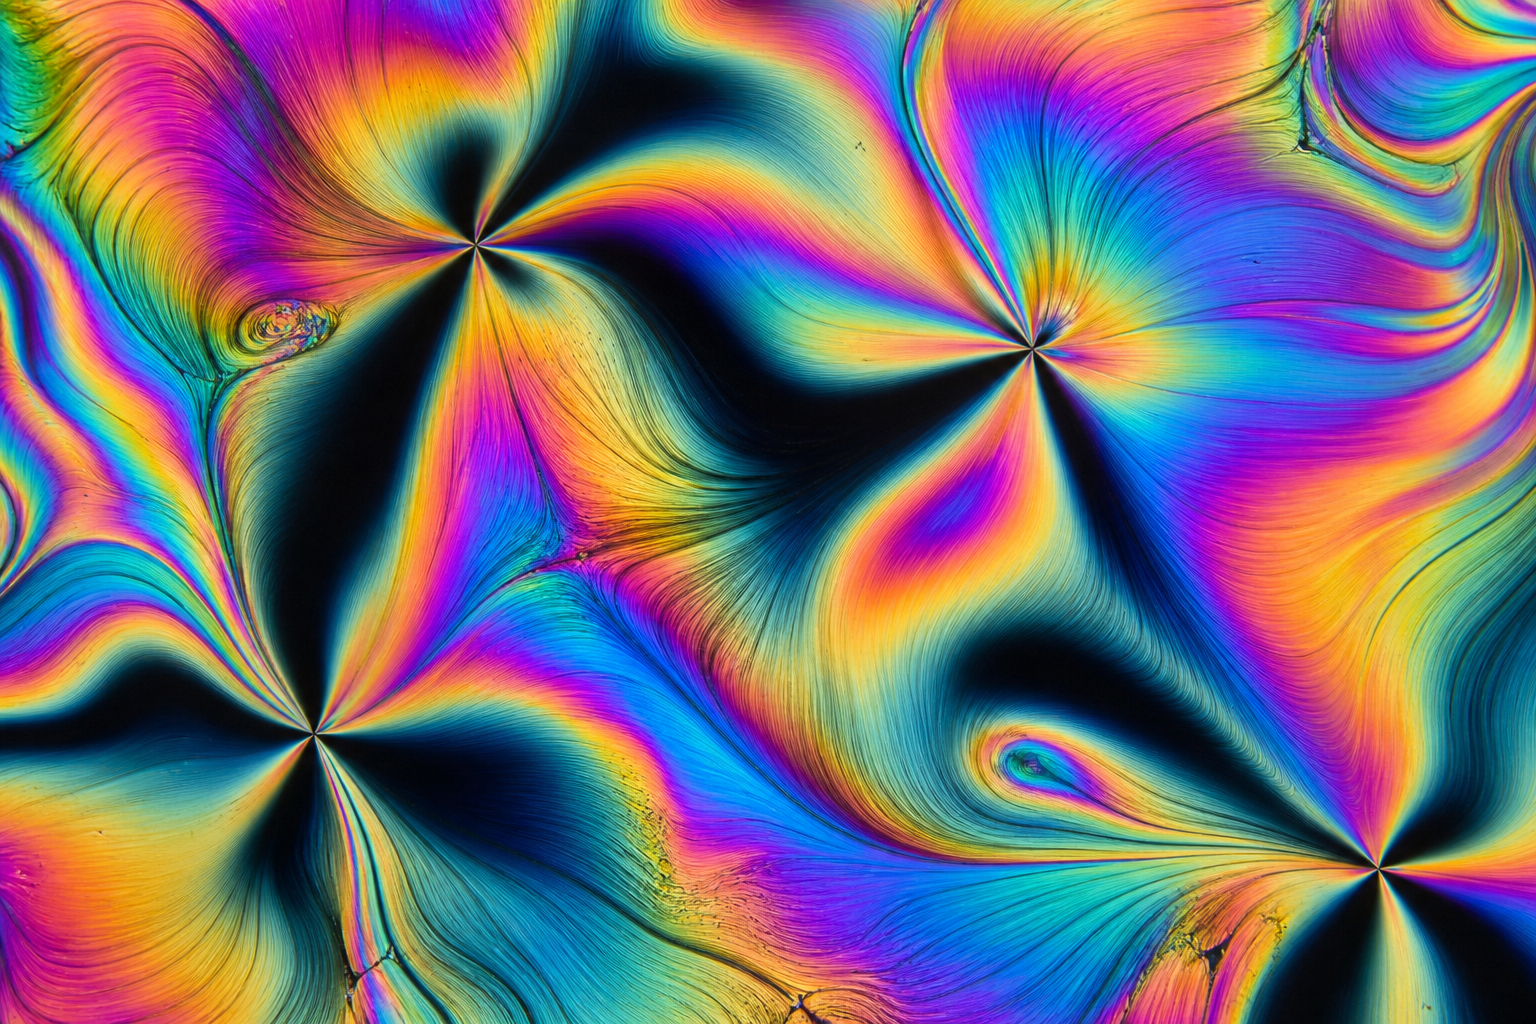
\includegraphics[width=0.58\linewidth]{images/book5/ai/b5-26-liquid-crystal.png}

{\small क्रॉस किए गए ध्रुवकों के बीच कोई द्रव क्रिस्टल: एक \omterm{def:b3:phase-transitions:order}{क्रम-प्राचल} (आणविक अक्ष) उन दोषों के बीच घूमता हुआ, जहाँ ब्रुशें मिलती हैं। द्रव और ठोस के बीच पदार्थ की प्रावस्थाएँ --- और अधिकांश परदों का कार्यकारी पदार्थ।}
\end{omfigure}

\section{अभ्यास}

\begin{exercise}[$\star$]\label{exo:b3:phase-transitions:1}
वर्गीकृत कीजिए (प्रथम-कोटि या सतत), और \omterm{def:b3:phase-transitions:order}{क्रम-प्राचल} तथा भंग हुई
सममिति, यदि कोई हो, बताइए: (क) \qty{1}{atm} पर उबलना; (ख)
क्यूरी बिंदु; (ग) अतितरल $\lambda$ बिंदु; (घ) \emph{ठीक} \omterm{prop:b3:phase-transitions:vdw}{क्रांतिक
बिंदु} पर उबलना।
\end{exercise}

\begin{exercise}[$\star$]\label{exo:b3:phase-transitions:2}
गुप्त ऊष्माएँ, एन्ट्रॉपी के रूप में। (क) पानी: \qty{373}{K} पर
$L_{\text{वा}} =
\qty{2.26e6}{J/kg}$: प्रति अणु $\Delta S$ को
$k_{\text{B}}$ की इकाइयों में निकालिए। (ख) वही गलन के लिए
(\qty{273}{K} पर $L_{\text{गल}} = \qty{3.3e5}{J/kg}$)। (ग) अधिकांश
द्रव $\Delta S \approx 10$--$11\,k_{\text{B}}$ के साथ वाष्पित होते
हैं (ट्राउटन का नियम): वह संख्या मोटे तौर पर क्या गिनती है (किस
आयतन-अनुपात का $\ln$)? (घ) गलन की एन्ट्रॉपी-छलाँग उबलने वाली से
इतनी छोटी क्यों है?
\end{exercise}

\begin{exercise}[$\star$]\label{exo:b3:phase-transitions:3}
फ़ान डेर वाल्स के क्रांतिक नियतांक ($V_{\text{c}} = 3Nb$,
$k_{\text{B}}T_{\text{c}} = 8a/27b$, $P_{\text{c}} = a/27b^2$ ---
मान लीजिए)। (क) दिखाइए कि $P_{\text{c}}V_{\text{c}}/Nk_{\text{B}}T_{\text{
c}} = 3/8$, जो इस प्रतिरूप की एक सार्वभौमिक संख्या है; और मापे गए
मान $0.29$ के पास गुच्छित हैं --- टिप्पणी कीजिए। (ख) CO$_2$ के लिए
($T_{\text{c}} = \qty{304}{K}$, $P_{\text{c}} = \qty{73.8}{bar}$):
$a$ और $b$ निकालिए। (ग) $b$ से आणविक व्यास
आकलिए। (घ) कमरे के ताप पर CO$_2$ दाब के नीचे द्रवित हो जाती है,
जबकि कमरे के ताप की N$_2$ ($T_{\text{c}} =
\qty{126}{K}$) कभी नहीं --- क्यों?
\end{exercise}

\begin{exercise}[$\star$]\label{exo:b3:phase-transitions:4}
\omterm{def:b3:phase-transitions:order}{क्रम-प्राचल}, झटपट: एक-एक बताइए (क) किसी लौहचुंबक के लिए; (ख)
द्रव--गैस संक्रमण के लिए; (ग) \omterm{thm:b3:quantum-statistics:bec}{बोस--आइंस्टाइन संघनन} के लिए; (घ)
किसी प्रति-लौहचुंबक के लिए (दो उप-जालक --- कौन-सी राशि क्रमित होती
है, जबकि कुल चुंबकन शून्य ही रहता है?)।
\end{exercise}

\begin{exercise}[$\star\star$]\label{exo:b3:phase-transitions:5}
माध्य-क्षेत्र, हाथ से। (क) $m = \tanh(\beta qJm)$ व्युत्पन्न कीजिए,
अपने $q$ पड़ोसियों के औसत क्षेत्र में बैठे किसी चक्रण से। (ख)
दिखाइए कि कोई अशून्य हल ठीक तभी है जब $T < qJ/k_{\text{B}}$। (ग)
तीसरी कोटि तक प्रसार कीजिए और $m(T) \approx \sqrt{3(1 -
T/T_{\text{c}})}$ व्युत्पन्न कीजिए। (घ) लोहा: $T_{\text{c}} = \qty{1043}{K}$, $q =
8$: $J$ को eV में निकालिए और
\cref{exo:b3:identical-particles:12} के विनिमय-पैमाने से जाँचिए।
\end{exercise}

\begin{exercise}[$\star\star$]\label{exo:b3:phase-transitions:6}
क्यूरी--वाइस। कोई छोटा क्षेत्र जोड़िए: $m = \tanh[\beta(qJm + \mu B)]$।
(क) $T_{\text{c}}$ के ऊपर रैखिकीकरण कीजिए और $\chi = \partial
m/\partial B \propto 1/(T - T_{\text{c}})$ व्युत्पन्न कीजिए। (ख)
मुक्त-चक्रण वाले क्यूरी नियम से तुलिए: हर स्थिति में $1/\chi$ को $T$
के सामने आलेखित करने पर क्या मिलता है, और अंतःखंड लौहचुंबकीय
युग्मन की पहचान कैसे करता है? (ग) निकल की $1/\chi$ रेखा
\qty{631}{K} पर शून्य छूती है: व्याख्या कीजिए। (घ) किसी
प्रति-लौहचुंबक के लिए अंतःखंड \emph{ऋणात्मक} होता है: वह $J$ के
कौन-से चिह्न की चुगली करता है?
\end{exercise}

\begin{exercise}[$\star\star$]\label{exo:b3:phase-transitions:7}
क्लॉसियस--क्लापेरों काम पर। (क) \qty{100}{\celsius} पर पानी
($\Delta v = \qty{1.67}{m^3/kg}$): $\dd P/\dd T$ निकालिए। (ख)
$\dd\ln P/\dd T = Lm_{\text{w}}/k_{\text{B}}T^2$ का उपयोग करके
$P = \qty{0.7}{atm}$ (किसी \qty{3000}{m} की चोटी) पर उबलने का ताप
आकलिए। (ग) गलन: $\Delta v = \qty{-9.1e-5}{m^3/kg}$ और
$L = \qty{3.3e5}{J/kg}$ के साथ $\dd T/\dd P$ निकालिए, और वह दाब भी
जो बर्फ़ का गलनांक \qty{5}{K} नीचे लाए। (घ) \qty{30}{mm^2} के
फलक पर कोई \qty{70}{kg} का स्केटर: दाब और उससे होता गलनांक-खिसकाव
--- क्या दाब-गलन स्केटिंग समझा देता है? (क्या समझाता है: घर्षण और
सतही पूर्व-गलन।)
\end{exercise}

\begin{exercise}[$\star\star$]\label{exo:b3:phase-transitions:8}
लांडाउ की गणनाएँ। (क) $F = a(T - T_{\text{c}})m^2 +
bm^4$ को $T_{\text{c}}$ से नीचे न्यूनतम कीजिए। (ख) न्यूनतम पर $F$ निकालिए और
दिखाइए कि संक्रमण पर ऊष्माधारिता में एक परिमित \emph{छलाँग} $\Delta C =
a^2T_{\text{c}}/2b$ है। (ग) $C(T)$ का रेखाचित्र बनाइए:
माध्य-क्षेत्र की सीढ़ी बनाम हीलियम के $\lambda$ बिंदु का मापा गया
लगभग-लघुगणकीय शिखर --- असली उतार-चढ़ाव उसमें क्या जोड़ते हैं? (घ)
कोई क्षेत्र-पद $-hm$ जोड़िए: दिखाइए कि संक्रमण गोल पड़ जाता है ---
सममिति को भंग होने के लिए यथार्थ होना ही चाहिए।
\end{exercise}

\begin{exercise}[$\star\star$]\label{exo:b3:phase-transitions:9}
नाभिकन। किसी अतिसंतृप्त वाष्प में त्रिज्या $r$ की कोई बूँद
पिंडीय \omterm{prop:b3:canonical-ensemble:machine}{मुक्त ऊर्जा} $-\tfrac43\pi r^3\,n\,\delta\mu$ कमाती है पर
पृष्ठ तनाव $4\pi r^2\sigma$ चुकाती है। (क) दिखाइए कि रोधिका
$r^* = 2\sigma/n\,\delta\mu$ पर शिखर बनाती है। (ख) समझाइए: स्वच्छ
अतिसंतृप्त वाष्प और अतितप्त द्रव क्यों बने रहते हैं
(अर्धस्थायित्व), और धूल, आयन तथा खरोंचें क्या दे देती हैं?
(ग) मेघ-कक्ष (\cref{ch:b3:particle-physics} के पूर्वज संसूचक)
और बुलबुला-कक्ष इसी भौतिकी \emph{पर} चलते हैं: गुज़रते कण की
आयन-पगडंडी क्या भूमिका निभाती है? (घ) प्रयोगशाला के फ़्लास्कों में
``उबाल-कंकड़'' क्यों डाले जाते हैं?
\end{exercise}

\begin{exercise}[$\star\star\star$]\label{exo:b3:phase-transitions:10}
एक विमा में कोई संक्रमण नहीं। एक-विमीय आइज़िंग शृंखला लीजिए, जिसमें
$N$ चक्रण सब ऊपर हों, और एक ``प्रांत-दीवार'' डालिए (किसी बंध के आगे
सारे चक्रण पलट दिए गए)। (क) उस दीवार की ऊर्जा-लागत: $2J$,
जो स्थिति से स्वतंत्र है। (ख) एन्ट्रॉपी का लाभ: वह दीवार
$\sim N$ बंधों में से किसी पर भी बैठ सकती है --- $\Delta S = k_{\text{B}}\ln N$। (ग)
दिखाइए कि $\Delta F = 2J - k_{\text{B}}T\ln N < 0$ किसी भी $T > 0$ के
लिए, बड़े $N$ पर:
दीवारें सदा फैलती जाती हैं, और दीर्घ-परास क्रम असंभव है --- अर्थात्
एक-विमीय \omterm{thm:b3:phase-transitions:meanfield}{आइज़िंग प्रतिरूप} का $T_{\text{c}} = 0$ है। (घ) दो
विमाओं में कोई दीवार लंबाई $\ell$ की एक रेखा है, जिसकी लागत $2J\ell$
है पर जिसके $\sim3^\ell$ आकार हैं: आकलन दोहराइए और दिखाइए कि किसी
परिमित $T_{\text{c}}$ से नीचे क्रम \emph{बचा रहता} है --- यही
पाइर्ल्स का तर्क है, जो ओन्सागर के यथार्थ $2.269\,J/k_{\text{B}}$ के
पीछे है।
\end{exercise}

\begin{exercise}[$\star\star\star$]\label{exo:b3:phase-transitions:11}
सार्वभौमिकता की जाँच। माध्य-क्षेत्र $\beta = 1/2$, $\gamma
= 1$ ($\chi \sim |t|^{-\gamma}$), $\delta = 3$ ($m \sim h^{1/3}$,
$T_{\text{c}}$ पर) की भविष्यवाणी करता है। जबकि द्रव--गैस \omterm{prop:b3:phase-transitions:vdw}{क्रांतिक
बिंदु} \emph{और} त्रिविमीय एक-अक्षीय चुंबक, दोनों के लिए मापा गया: $\beta
\approx 0.326$, $\gamma \approx 1.237$, $\delta \approx 4.79$।
(क) किसी तरल की किसी चुंबक से तुलना करना उचित ही क्यों है (उनके
\omterm{def:b3:phase-transitions:order}{क्रम-प्राचल} क्या साझा करते हैं --- एक ही चिह्न-चुनाव)? (ख)
माध्य-क्षेत्र $T_{\text{c}}$ के पास विफल क्यों होता है (क्या
अपसरित होता है, जिससे उतार-चढ़ावों की उपेक्षा अवैध हो जाती है)? (ग)
ऊँची विमाओं में वह \emph{कम} विफल क्यों होता है (पड़ोसियों की
संख्या बनाम उतार-चढ़ाव की पहुँच; चार विमाओं के ऊपर माध्य-क्षेत्र
यथार्थ हो जाता है)? (घ) दो वाक्यों में पुनर्प्रसामान्यन समूह का सार
बताइए: पैमाने-दर-पैमाने किसका औसत लिया जा रहा है, और उस औसत से केवल
सममिति और विमा ही क्यों बचती हैं।
\end{exercise}

\begin{exercise}[$\star\star\star$]\label{exo:b3:phase-transitions:12}
चुंबकों से हिग्स तक। \omterm{def:b3:phase-transitions:order}{क्रम-प्राचल} को किसी क्षेत्र
$\phi(\vect r)$ तक पदोन्नत कीजिए, जिसका लांडाउ ऊर्जा घनत्व $\alpha(T -
T_{\text{c}})\phi^2 + b\phi^4$ हो, साथ में एक प्रवणता-पद। (क)
$T_{\text{c}}$ से नीचे वह क्षेत्र $\pm\phi_0$ पर बैठता है: कूप के
\emph{अनुदिश} छोटे दोलनों में एक प्रत्यानयन वक्रता होती है ---
$F''(\phi_0)$ निकालिए और क्षेत्र की भाषा में उसकी व्याख्या किसी
\emph{द्रव्यमान} के रूप में कीजिए। (ख) किसी \emph{सम्मिश्र}
\omterm{def:b3:phase-transitions:order}{क्रम-प्राचल} के लिए (न्यूनतमों का एक वृत्त --- ``मेक्सिकन टोप''),
किनारे के \emph{चारों ओर} के दोलनों की कोई स्थितिज ऊर्जा नहीं लगती:
यानी एक द्रव्यमानहीन मोड --- उसके संघनित-पदार्थ समरूपों के नाम
लीजिए (चक्रण-तरंगें, अतितरल फ़ोनॉन)। (ग)
विद्युत्दुर्बल सिद्धांत में स्वयं निर्वात ऐसे ही \omterm{def:b3:phase-transitions:order}{सममिति-भंग} वाले
कूप में बैठा है; कण उस क्षेत्र के अशून्य मान से द्रव्यमान पाते हैं,
और त्रिज्य दोलन \emph{ही} हिग्स
बोसॉन है: हर अवयव को (क)--(ख) पर मानचित्रित कीजिए। (घ) एक वाक्य
में: यहाँ संघनित-पदार्थ भौतिकी ने कण भौतिकी को क्या सिखाया
(ऐंडरसन के ज़रिए \omterm{def:b3:phase-transitions:order}{सममिति-भंग} का निर्यात)?
\end{exercise}

\begin{omfigure}
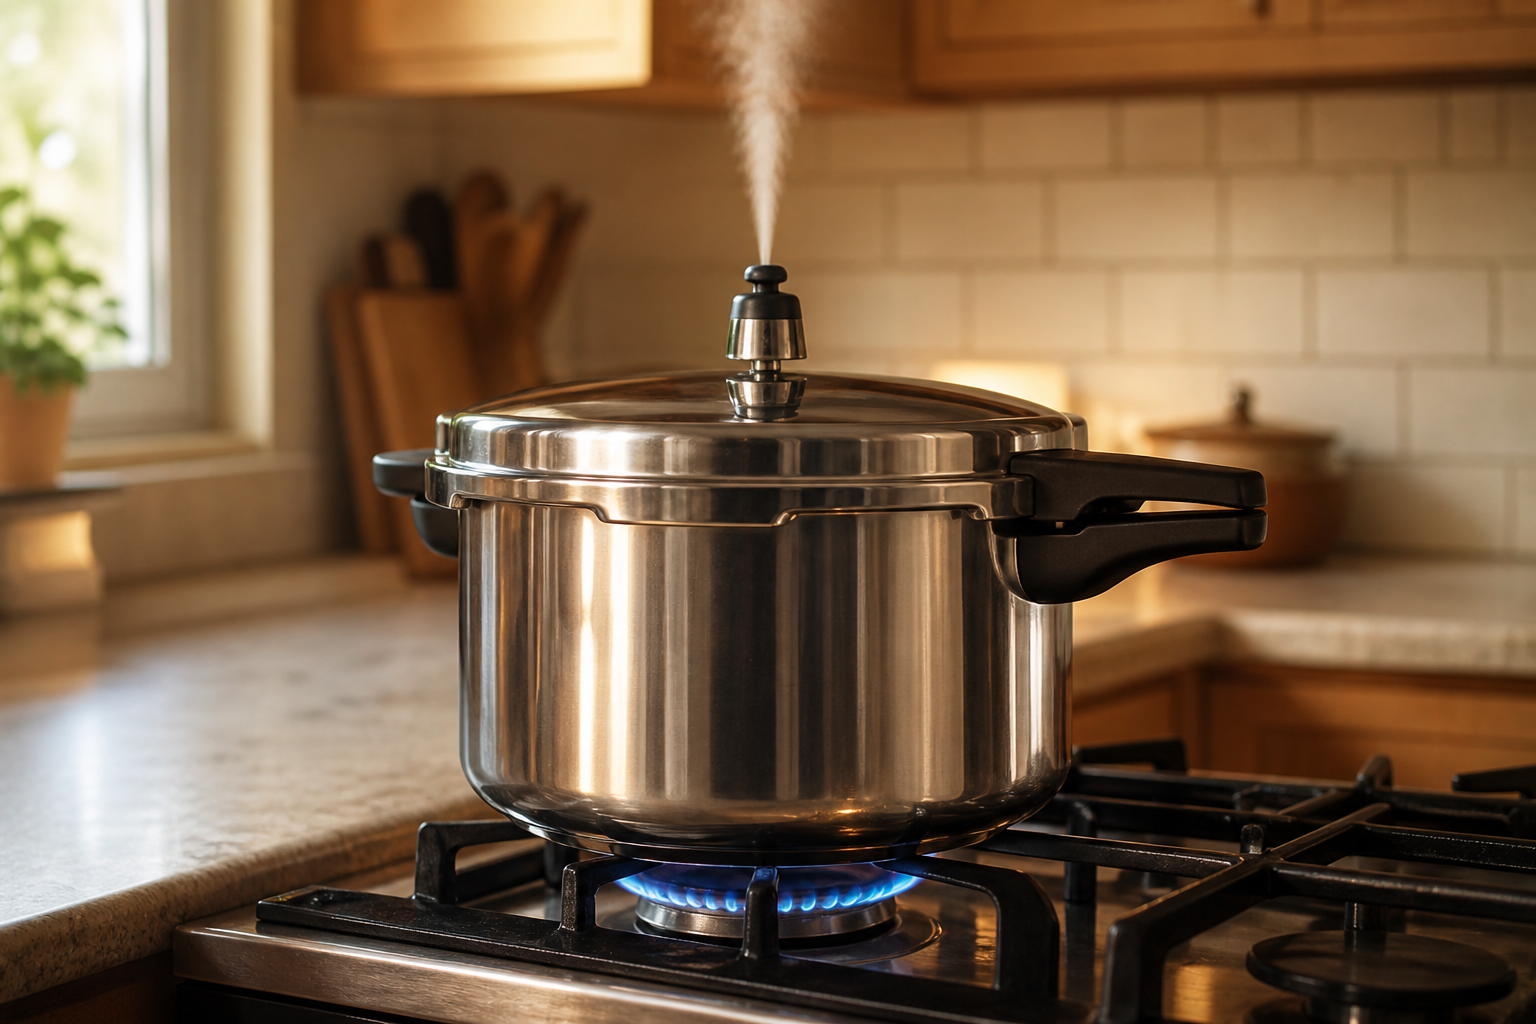
\includegraphics[width=0.58\linewidth]{images/book5/ai/b5-17-pressure-cooker.png}

{\small भाप छोड़ता एक प्रेशर कुकर: भीतर के दो वायुमंडल द्रव--वाष्प सह-अस्तित्व रेखा को \qty{121}{\celsius} तक खिसका देते हैं --- क्लॉसियस और क्लापेरों, रात का खाना तेज़ी से पकाते हुए।}
\end{omfigure}

\section{समस्या: रसोई का प्रावस्था-आरेख}

\begin{problem}[{सप्ताहांत समस्या --- प्रेशर कुकर, पहाड़ी चाय,
और उबलने का अंत}]\label{pb:b3:phase-transitions:1}
पानी का प्रावस्था-आरेख हर चूल्हे के ऊपर टँगा रहता है, बिना ध्यान
खींचे। यह समस्या क्लॉसियस--क्लापेरों को हाथ में लेकर उसकी तीनों
रेखाओं पर चलती है --- प्रेशर कुकर पकाने का समय आधा क्यों कर देता है,
से लेकर ऊँचाई पर चाय क्यों निराश करती है, और उस अजीब संसार तक जहाँ
\omterm{prop:b3:phase-transitions:vdw}{क्रांतिक बिंदु} के आगे उबलना ही समाप्त हो जाता है। आँकड़े: $L_{\text{वा}}
= \qty{2.26e6}{J/kg}$, $L_{\text{गल}} = \qty{3.34e5}{J/kg}$;
\qty{373}{K}, \qty{1}{atm} पर जल-वाष्प: $\Delta v_{\text{वा}}
= \qty{1.67}{m^3/kg}$; गलन: $\Delta v = \qty{-9.1e-5}{m^3/kg}$;
आणविक द्रव्यमान $m_{\text{w}} = \qty{3.0e-26}{kg}$; \omterm{prop:b3:phase-transitions:vdw}{क्रांतिक बिंदु}:
$T_{\text{c}} = \qty{647}{K}$, $P_{\text{c}} = \qty{221}{bar}$।

\medskip\noindent\textbf{भाग I --- उबलने की रेखा।}
\begin{enumerate}
  \item किसी दिए गए दाब पर ``उबलना'' किससे परिभाषित होता है (कौन-से
        दो \omterm{thm:b3:grand-canonical:distribution}{रासायनिक विभव} बराबर होते हैं)?
  \item \qty{100}{\celsius} पर वाष्पन रेखा की ढाल $\dd P/\dd T$
        निकालिए।
  \item कोई प्रेशर कुकर \qty{2}{atm} रखता है: ढाल को समाकलित
        कीजिए (या चरघातांकी रूप को $Lm_{\text{w}}/
        k_{\text{B}} \approx \qty{4900}{K}$ के साथ काम में लीजिए)
        और उसके उबलने का ताप खोजिए।
  \item \cref{exo:b3:canonical-ensemble:9} के आरेनियस-रसोई नियम
        (हर \qty{10}{K} पर दर दुगनी) के साथ खुले बर्तन में पकाने
        की तुलना में तेज़ी का आकलन कीजिए।
  \item ला पाज़ में (\qty{3600}{m}, $P \approx \qty{0.65}{atm}$):
        उबलने का ताप, और चाय क्यों खराब बनती है।
  \item नमक डालने से क्वथनांक क्यों चढ़ जाता है (विलेय किसका $\mu$
        घटाता है --- \cref{exo:b3:grand-canonical:8} याद
        कीजिए)?
\end{enumerate}

\medskip\noindent\textbf{भाग II --- गलन की रेखा।}
\begin{enumerate}[resume]
  \item गलन के लिए $\dd T/\dd P$ निकालिए और उसका चिह्न देखिए।
  \item रोज़ का कौन-सा प्रेक्षण $\Delta v < 0$ को समेटे है (आपके
        गिलास में बर्फ़ क्या करती है), और वह विषमता पदार्थों में
        इतनी दुर्लभ क्यों है?
  \item \qty{300}{m} मोटा कोई हिमनद: उसके तल पर दाब और गलनांक का
        अवनमन --- क्या तली का दाब-गलन हिमनद के बहाव के लिए मायने
        रखता है?
  \item \cref{exo:b3:phase-transitions:7}(घ) के स्केटर पर फिर से
        लौटिए: फलक को वस्तुतः चिकना कौन बनाता है?
  \item यदि बर्फ़ डूबती (धनात्मक ढाल, लगभग हर दूसरे ठोस की तरह),
        तो सर्दियाँ झीलों और उनकी मछलियों का क्या करतीं ---
        परिणामों की शृंखला बताइए।
  \item वह ऋणात्मक ढाल ऊँचे दाब पर समाप्त हो जाती है, जहाँ बर्फ़
        के दूसरे क्रिस्टल-रूप कमान ले लेते हैं (बर्फ़ III, V, VI):
        एक ही सरल अणु की एक दर्जन बर्फ़ों का होना उसके मुक्त-ऊर्जा
        भूदृश्य के बारे में क्या कहता है?
\end{enumerate}

\medskip\noindent\textbf{भाग III --- रेखा का अंत।}
\begin{enumerate}[resume]
  \item उबलने की रेखा ($T_{\text{c}},
        P_{\text{c}}$) पर समाप्त होती है: उस अंत के पास पहुँचने पर
        गुप्त ऊष्मा और घनत्व-अंतर का क्या होता है?
  \item \omterm{prop:b3:phase-transitions:vdw}{क्रांतिक बिंदु} के आगे पानी को ``द्रव-सरीखे'' से
        ``गैस-सरीखे'' तक बिना \emph{किसी} संक्रमण के ले जाया जा
        सकता है: $(P, T)$ तल में उस पथ का वर्णन कीजिए।
  \item \omterm{prop:b3:phase-transitions:vdw}{क्रांतिक बिंदु} के पास पहुँचने पर तरल दूधिया हो जाता है:
        इस दुग्धाभा को
        \cref{exo:b3:microcanonical-ensemble:12} और
        \cref{pb:b3:perturbation-theory:1} से जोड़िए।
  \item अतिक्रांतिक CO$_2$ ($T_{\text{c}} = \qty{304}{K}$,
        $P_{\text{c}} = \qty{74}{bar}$) द्रव की तरह घोलती है और
        गैस की तरह भीतर घुसती है: उस औद्योगिक उपयोग का नाम लीजिए
        जो कॉफ़ी से कैफ़ीन हटाता है, और यह भी कि वह विलायक कोई
        अवशेष क्यों नहीं छोड़ता।
  \item अतिक्रांतिक पानी (\qty{221}{bar} से ऊपर बिजलीघरों के
        बॉयलरों में): उबलना --- बुलबुले, फ़िल्में, जलना --- मिटा
        देना बॉयलर अभियंताओं को क्यों भाता है?
  \item गहरे समुद्र के तापजलीय छिद्र \qty{400}{\celsius} का पानी
        उगलते हैं, जो उबलता नहीं: स्थानीय दाब
        (\qty{3}{km} पर $\sim\qty{300}{bar}$) और प्रावस्था-आरेख के
        सामने जाँचिए।
\end{enumerate}

\medskip\noindent\textbf{भाग IV --- पूरा नक्शा पढ़ना।}
\begin{enumerate}[resume]
  \item शब्दों में पानी का $(P, T)$ आरेख खींचिए: तीनों
        रेखाएँ, त्रिक बिंदु ($\qty{0.01}{\celsius}$,
        \qty{611}{Pa}), और \omterm{prop:b3:phase-transitions:vdw}{क्रांतिक बिंदु}।
  \item \qty{611}{Pa} से नीचे बर्फ़ बिना गले ऊर्ध्वपातित हो जाती
        है: कौन-सा उपकरण (हिम-शुष्कन) और किस ग्रह की ध्रुवीय
        टोपियाँ (मंगल, CO$_2$ और H$_2$O) इसी तथ्य पर जीते हैं?
  \item पानी का त्रिक बिंदु --- जो 2019 तक परिभाषा से ठीक
        \qty{273.16}{K} था --- इतना अच्छा ताप-मानक क्यों था
        (कितनी सह-अस्तित्व वाली प्रावस्थाएँ कितनी
        स्वातंत्र्य कोटियाँ बाँध देती हैं)?
  \item नक्शे की हर रेखा एक प्रथम-कोटि संक्रमण है; केवल उसका
        अंत-बिंदु क्रांतिक है: इस भेद को
        \omterm{def:b3:phase-transitions:order}{क्रम-प्राचल} और गुप्त ऊष्मा से फिर कहिए।
  \item आर्द्र हवा की ओस-रेखा वही भौतिकी उलटी चलाई हुई है: ओस,
        कुहरा और ठंडी खिड़की पर सुबह की धुंध को एक $\mu$-कटान वाले
        वाक्य से समझाइए।
  \item हर बर्तन का ढक्कन एक प्रयोग है: उस पर बूँदें संघनित होती
        हैं और वापस बरसती हैं --- उस लघु जलचक्र के दोनों
        \omterm{def:b3:phase-transitions:order}{प्रावस्था संक्रमण} पहचानिए, और वह गुप्त-ऊष्मा की फेरी भी,
        जिससे ढका बर्तन जल्दी उबलता है।
  \item नामित परिणाम का सार दीजिए: एक ही ढाल-सूत्र, $\dd P/
        \dd T = L/T\Delta v$, प्रेशर कुकर के
        \qty{121}{\celsius}, पहाड़ की \qty{88}{\celsius} वाली
        चाय, अपनी गलन-रेखा पर उलटी चढ़ती तैरती बर्फ़, और उस
        अतिक्रांतिक केतली को समझा देता है जहाँ उबलना
        $\qty{647}{K}, \qty{221}{bar}$ पर समाप्त हो जाता है।
\end{enumerate}
\end{problem}
